\documentclass[
    11pt,
    aspectratio=169,
]{beamer}

\usepackage{graphicx}
\graphicspath{{images/}}
\usepackage{booktabs}
\usepackage{array}
\usepackage{tikz}
\usetikzlibrary{shapes.geometric, shapes.misc, shapes.symbols, arrows.meta, positioning, calc, decorations.pathmorphing}

%%% Citations
\usepackage[style=authoryear, backend=bibtex]{biblatex}
\addbibresource{references.bib}

%%% Customize Theme %%%%%%%%%%%%%%%%%%%%%%
\usetheme{Madrid}

\definecolor{myRed}{RGB}{134,31,65}
\definecolor{myOrange}{RGB}{229, 117, 31}

\setbeamercolor*{structure}{bg=myRed!20,fg=myRed!90}
\setbeamercolor*{palette primary}{use=structure,fg=white,bg=structure.fg}
\setbeamercolor*{palette secondary}{use=structure,fg=myRed,bg=white}
\setbeamercolor*{palette tertiary}{use=structure,fg=white,bg=myRed}
\setbeamercolor{frametitle}{bg=myRed!85,fg=white}
\setbeamercolor*{titlelike}{parent=palette primary}
\setbeamercolor{section in head/foot}{fg=myOrange, bg=white}

%%% Specific Colors %%%
\setbeamercolor{item projected}{bg=myOrange}
\setbeamertemplate{enumerate items}{bg=myOrange}
\setbeamercolor{itemize item}{fg=myOrange}
\setbeamercolor{itemize subitem}{fg=myOrange}
\setbeamercolor{button}{bg=myOrange}

%%% TOC %%%
\setbeamercolor{section in toc}{fg=black}
\setbeamercolor{subsection in toc}{fg=black}

%%% Block Colors %%%
\setbeamercolor{block title}{bg=myOrange, fg=white}
\setbeamercolor{block body}{bg=myOrange!20}
\setbeamercolor{block title alerted}{bg=myOrange!90, fg=white}
\setbeamercolor{block body alerted}{bg=myOrange!15}

\ifdefined\shownotes
  \usepackage{pgfpages}
  \setbeameroption{show notes on second screen=right}
\fi

%---------------------------------------------------------
%	FONT THEME & FONTS
%---------------------------------------------------------
\usefonttheme{default}
\usepackage{palatino}
\usepackage[default]{opensans}
\useinnertheme{circles}

%---------------------------------------------------------
%	OUTER THEME
%---------------------------------------------------------
\useoutertheme{miniframes}

%---------------------------------------------------------
%	PRESENTATION INFORMATION
%---------------------------------------------------------

\title[VT PhD Qualifier]{Agentic Knowledge Graphs for\\Research Progression}
\subtitle{PhD Qualifying Exam Presentation}
\author[J. Cusati]{Jason Cusati}
\institute[Virginia Tech]{Department of Computer Science \\ Virginia Tech \\ \smallskip \textit{djjay@vt.edu}}
\date[Spring 2026]{Spring 2026}

%--- Logo in frametitle (top right) ---%
\setbeamertemplate{frametitle}{%
  \nointerlineskip%
  \vskip-2pt%
  \begin{beamercolorbox}[wd=\paperwidth, sep=4pt, leftskip=0.3cm, rightskip=0pt]{frametitle}%
    \usebeamerfont{frametitle}\insertframetitle\hfill%
    \raisebox{-0.05cm}{
\includegraphics[height=0.55cm]{vt_logo_horiz.jpg}}%
  \end{beamercolorbox}%
}

%---------------------------------------------------------
%---------------------------------------------------------
\begin{document}

%---------------------------------------------------------
%	TITLE SLIDE
%---------------------------------------------------------
\section{}
\begin{frame}
	\titlepage

	\note{
Good morning. I'm Jason Cusati, a PhD student working with Dr.\ Brown at the Code World No Blanket Lab here at Virginia Tech. The lab name is fitting, actually --- today I'm arguing that AI research systems need somewhere to put their knowledge, because right now they're working without a net. Or a blanket. Today's talk is Agentic Knowledge Graphs for Research Progression --- the academic way of saying: what if AI actually remembered what it learned, and could connect the dots --- not just within a single paper, but across a whole field of research?
	}
\end{frame}

%---------------------------------------------------------
%	TABLE OF CONTENTS
%---------------------------------------------------------
\begin{frame}
	\frametitle{Outline}
	\tableofcontents

	\note{
Here's the plan for the next 15 minutes. I'll start with the problem --- why current AI-assisted workflows keep starting from scratch. Then I'll survey five domains and show where the gaps are. From there I'll present the proposal: a provenance-first architecture that gives agents a persistent, structured memory. I'll close with the evaluation framework and contributions. Questions at the end --- I'm told there will be some, so I've been practicing my nervous smile.
	}
\end{frame}

%---------------------------------------------------------
%	SECTION 1: MOTIVATION
%---------------------------------------------------------
\section{Motivation}

%--- Slide 1: The Structural Problem in AI-Assisted Research ---
\begin{frame}{The Structural Problem in AI-Assisted Research}

\begin{columns}[c]
	\begin{column}{0.5\textwidth}
		\begin{itemize}
			\item Research reasoning is \textbf{fragmented} and \textbf{transient}\newline
			\item LLM-assisted workflows \textbf{amplify volatility}\newline
			\item \textbf{Structural memory} is missing
		\end{itemize}
	\end{column}
	\begin{column}{0.47\textwidth}
		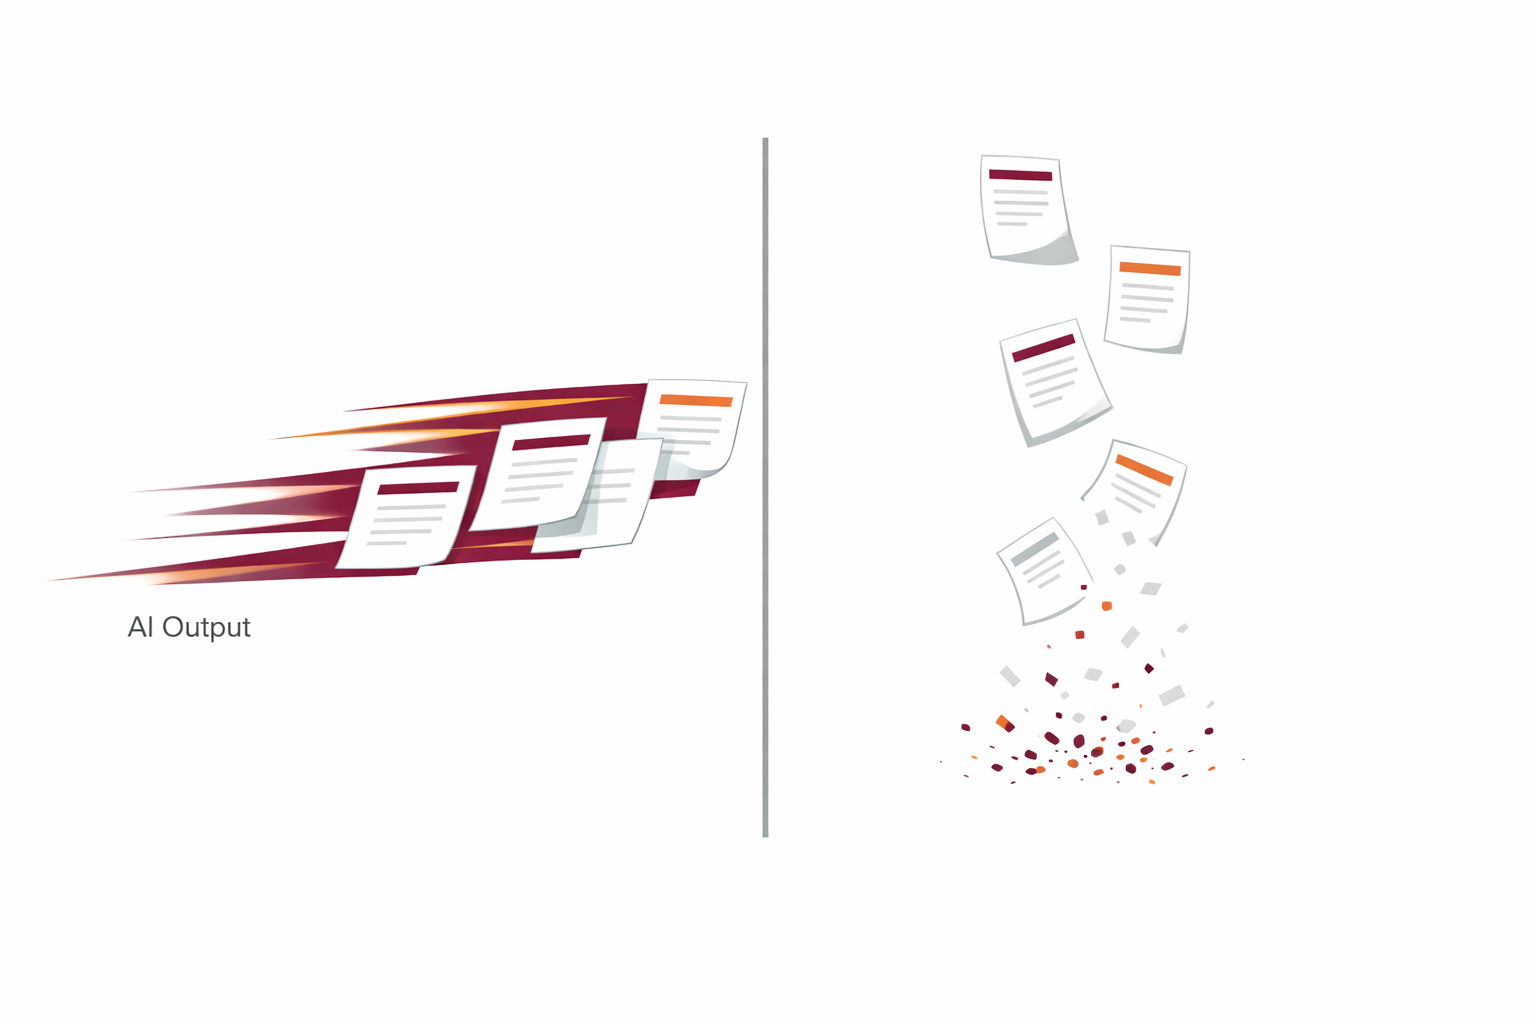
\includegraphics[width=\linewidth]{ai_research_state_problem.png}
	\end{column}
\end{columns}

\note{
Current AI systems dramatically accelerate document generation and research exploration.

However, they do not accumulate structured, validated, provenance-aware knowledge across iterations.

Outputs are transient. Each interaction effectively starts from scratch.

This work investigates how agentic systems combined with knowledge graphs can provide a persistent substrate for research progression.
}

\end{frame}

%--- Slide 2: The Structural Gaps ---
\begin{frame}
	\frametitle{The Structural Gaps}

	\begin{columns}[c]
		\begin{column}{0.6\textwidth}
			\begin{itemize}
				\item \textbf{Persistence:} State beyond session boundaries\newline
				\item \textbf{Traceability:} Linkage from Claim $\to$ Evidence\newline
				\item \textbf{Evaluability:} Empirical measurement of progression
			\end{itemize}
		\end{column}
		\begin{column}{0.35\textwidth}
			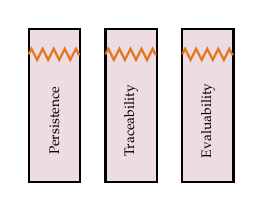
\begin{tikzpicture}[scale=0.65]
				% Three pillars
				\foreach \x/\label in {0/P, 1.5/T, 3/E} {
					\draw[thick, fill=myRed!15] (\x,0) rectangle (\x+1,3);
					\draw[thick, myOrange, decorate, decoration={zigzag, segment length=4, amplitude=2}] (\x,2.5) -- (\x+1,2.5);
				}
				\node[rotate=90] at (0.5,1.2) {\tiny Persistence};
				\node[rotate=90] at (2,1.2) {\tiny Traceability};
				\node[rotate=90] at (3.5,1.2) {\tiny Evaluability};
			\end{tikzpicture}
		\end{column}
	\end{columns}

	\vspace{0.5em}
	\begin{center}
		\emph{These are infrastructure problems, not model-quality problems.}
	\end{center}

	\note{
This manifests as three specific structural gaps.

First, Persistence: We lack state that survives beyond a single chat session.
Second, Traceability: When an agent makes a claim, we often cannot trace it back to the specific evidence that supported it.
Third, Evaluability: We lack the tools to empirically measure if our research knowledge is actually progressing over time.

Crucially, these are infrastructure problems, not model quality problems. Better models won't fix this --- better architecture will.
	}
\end{frame}

%--- Slide 3: Guiding Question ---
\begin{frame}
	\frametitle{Guiding Question}

	\vspace{1.5em}
	\begin{center}
		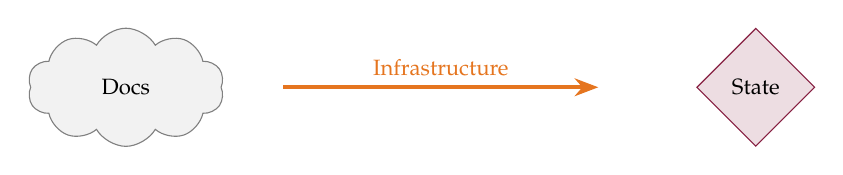
\begin{tikzpicture}
			% Chaotic docs
			\node[cloud, draw=gray, fill=gray!10, cloud puffs=10, cloud puff arc=120, minimum width=2.5cm, minimum height=1.5cm] (chaos) at (0,0) {\footnotesize Docs};
			% Bridge
			\draw[-{Stealth[length=3mm]}, ultra thick, myOrange] (2,0) -- node[above]{\footnotesize Infrastructure} (6,0);
			% Structured crystal
			\node[diamond, draw=myRed, fill=myRed!15, minimum width=1.5cm, minimum height=1.5cm] (crystal) at (8,0) {\footnotesize State};
		\end{tikzpicture}
	\end{center}

	\vspace{1em}
	\begin{block}{}
		\centering
		\textbf{How can research state be made persistent, traceable, and empirically evaluable in AI-assisted workflows?}
	\end{block}

	\note{
This leads to the guiding question of my proposal:

How can we transform this ephemeral interaction into something solid? How can research state be made persistent, traceable, and empirically evaluable in AI-assisted workflows?

To answer this, I've surveyed the current landscape to understand what pieces we already have --- and what is missing.
	}
\end{frame}

%---------------------------------------------------------
%	SECTION 2: LITERATURE SURVEY
%---------------------------------------------------------
\section{Literature Survey}

%--- Slide 4: Landscape Overview ---
\begin{frame}
	\frametitle{Landscape Overview}

	\begin{center}
		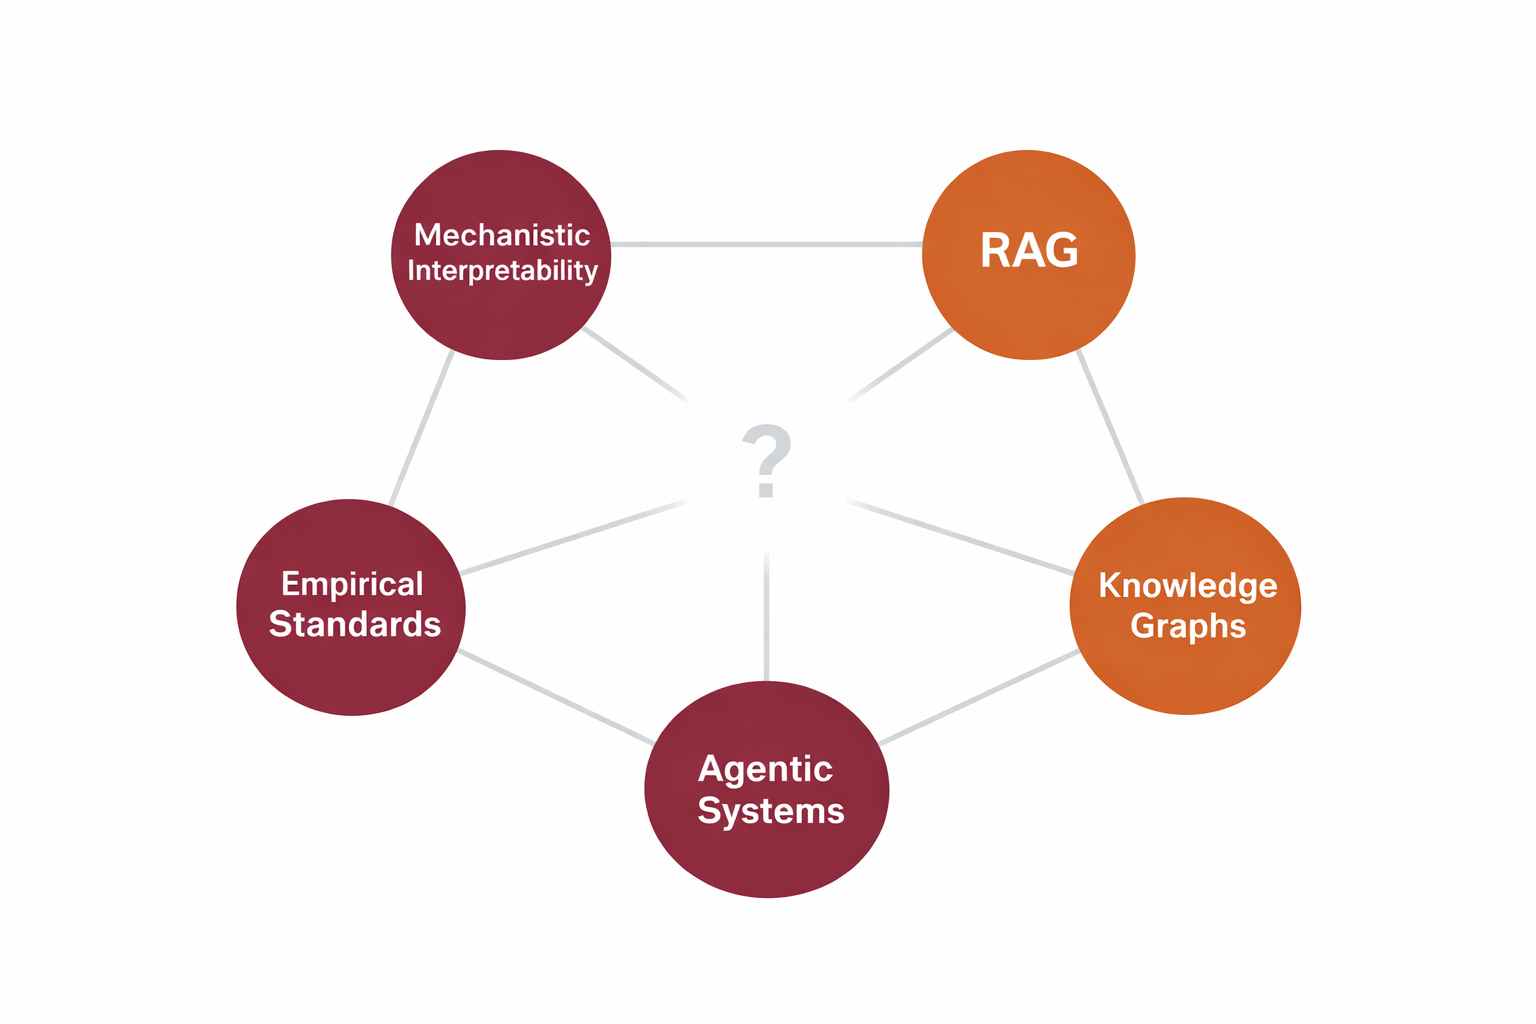
\includegraphics[height=0.72\textheight, keepaspectratio]{landscape_overview.png}
	\end{center}

	\note{
I surveyed five key domains that contribute to this problem.

We look at Mechanistic Interpretability to understand how models represent knowledge internally.
We look at RAG and Knowledge Graphs as two ways of representing knowledge externally.
We look at Agentic Systems which act on that knowledge.
And finally, Empirical Standards to understand how we should evaluate these systems.
	}
\end{frame}

%--- Slide 5: Mechanistic Interpretability ---
\begin{frame}
	\frametitle{Mechanistic Interpretability}

	\begin{columns}[c]
		\begin{column}{0.46\textwidth}
			\begin{itemize}
				\setlength{\itemsep}{6pt}
				\item Reverse-engineer the black box \textbf{\footcite{sharkey2025mechanistic}}
				\item Sparse features $\to$ human-interpretable structure
				\item Tells us \emph{how} a model thinks
			\end{itemize}
			\vspace{0.6em}
			\begin{alertblock}{Limitation}
				\small Static weights only --- no writable memory for new research state.
			\end{alertblock}
		\end{column}
		\begin{column}{0.50\textwidth}
			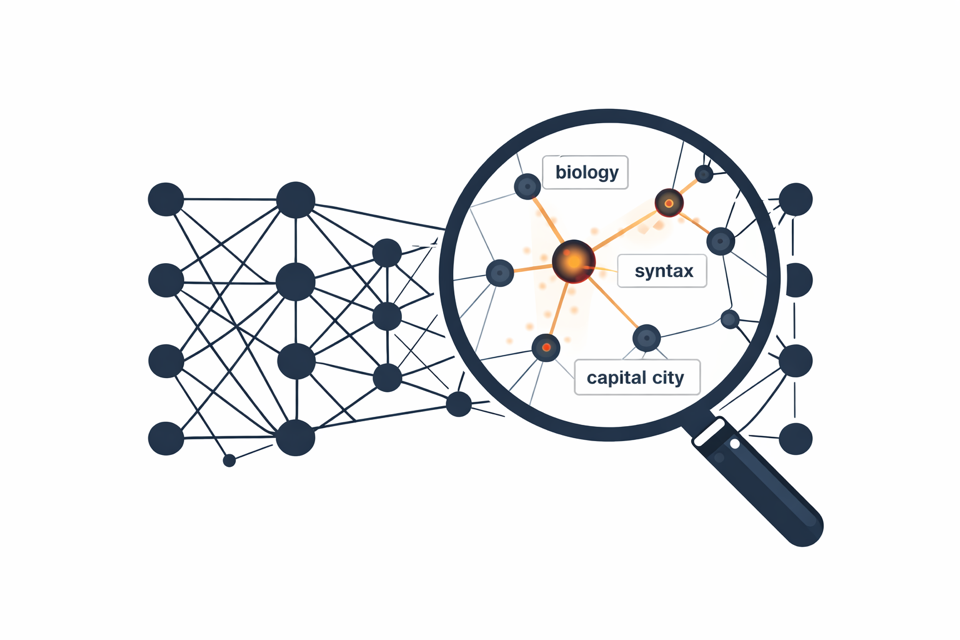
\includegraphics[width=\linewidth]{mechanistic_interpretability.png}
		\end{column}
	\end{columns}

	\note{
Starting with Mechanistic Interpretability, work by Sharkey et al. focuses on reverse-engineering the black box.

Techniques like sparse dictionary learning allow us to decompose model weights into understandable features. This is critical for understanding how a model thinks.

However, the limitation is that this focuses on the model's internal, static weights. It does not provide a mechanism for storing new research state that an agent generates during a workflow.
	}
\end{frame}

%--- Slide 6: Concept-Based Interpretability ---
\begin{frame}
	\frametitle{Concept-Based Interpretability}

	\begin{columns}[c]
		\begin{column}{0.65\textwidth}
			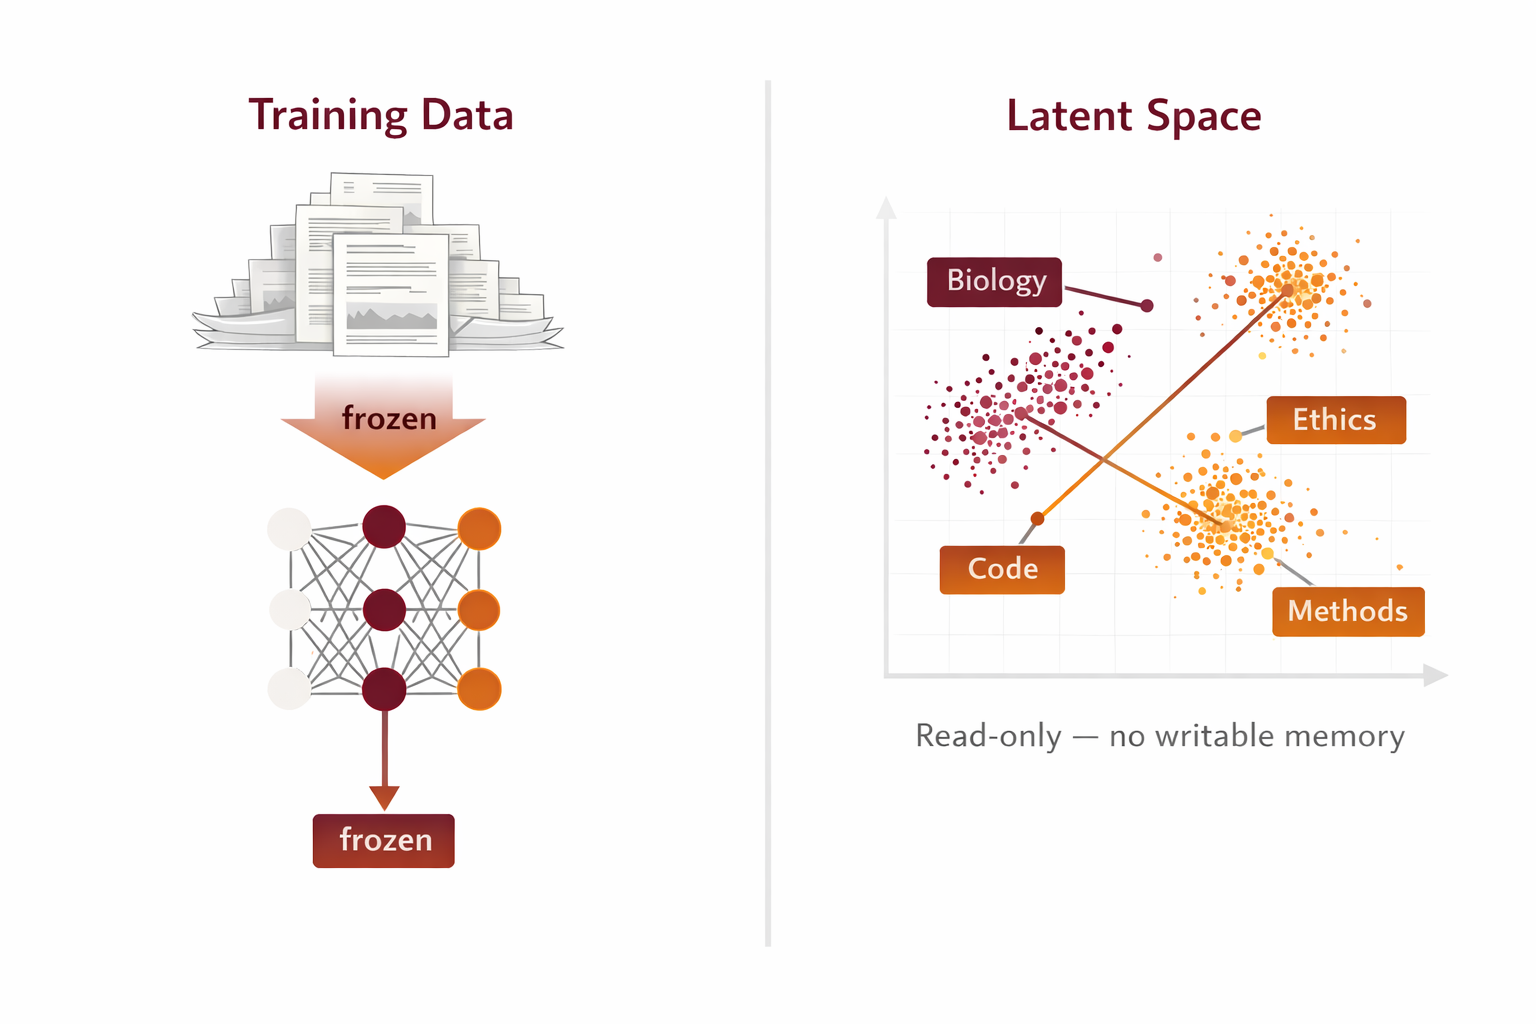
\includegraphics[width=\linewidth]{concept_interpretability.png}
		\end{column}
		\begin{column}{0.32\textwidth}
			\begin{alertblock}{Limitation}
				\small Read-only --- no mechanism to encode new research state.
			\end{alertblock}
		\end{column}
	\end{columns}

	\note{
Concept-based interpretability takes a different angle. Instead of looking at circuits and weights, it asks: can we find directions in the model's latent space that align with human-readable concepts --- like ``Biology'' or ``Code''?

And the answer is kind of yes. Probes can find those directions. But what we're really measuring is what the model learned from its training data. It's sophisticated pattern matching on frozen knowledge.

The problem is that probing is fundamentally read-only. It tells us what the model baked in during training --- not what we discovered in this session. Close the tab, and it's gone.
	}
\end{frame}

%--- Slide 7: RAG & Vector Memory Systems ---
\begin{frame}
	\frametitle{RAG \& Vector Memory Systems}

	\begin{columns}[c]
		\begin{column}{0.63\textwidth}
			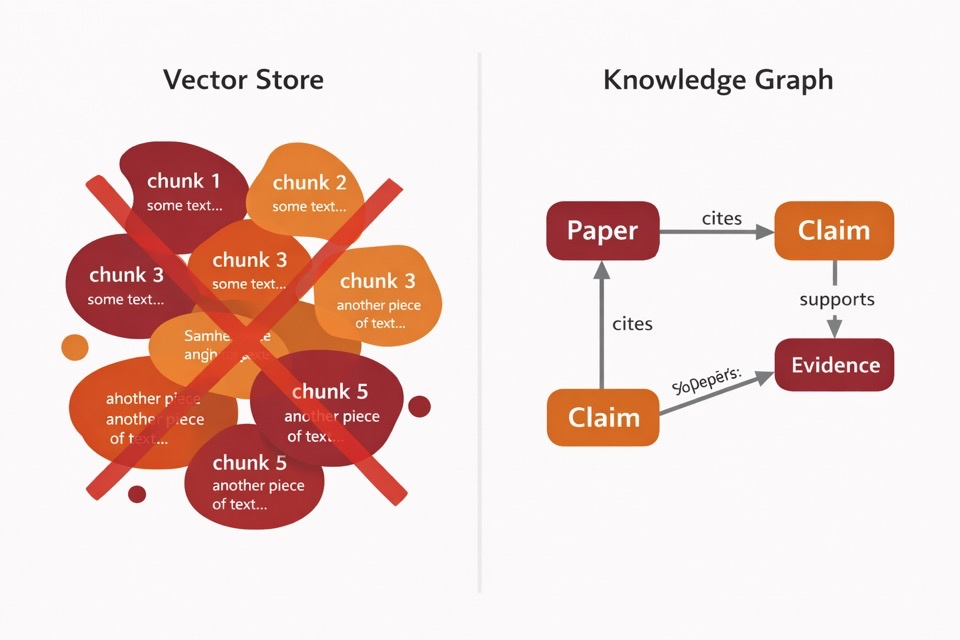
\includegraphics[width=\linewidth]{rag_vs_kg.jpg}
		\end{column}
		\begin{column}{0.34\textwidth}
			\begin{alertblock}{Limitations \footcite{suryawanshi2025kgrag}}
				\begin{itemize}
					\setlength{\itemsep}{4pt}
					\item No canonical memory
					\item No provenance chain
					\item No structured reasoning
					\item No longitudinal state
				\end{itemize}
			\end{alertblock}
		\end{column}
	\end{columns}

	\note{
RAG is the go-to for external memory right now, and for good reason --- it scales, it's fast, and semantic similarity gets you surprisingly far.

But Suryawanshi et al. point out the ceiling: vector retrieval gives you chunks, not structure. Similarity, not reasoning.

And critically, there's no canonical memory. Ask the same question after new papers drop and you get a different answer. No provenance chain --- you can't trace a generated claim back to the specific text that justified it.
	}
\end{frame}

%--- Slide 8: Knowledge Graph Research ---
\begin{frame}
	\frametitle{Knowledge Graph Research}

	\begin{columns}[t]
		\begin{column}{0.45\textwidth}
			\begin{block}{Strengths}
				\begin{itemize}
					\item Ontology-based structure
					\item Provenance modeling
					\item Logical relationships
				\end{itemize}
			\end{block}
		\end{column}
		\begin{column}{0.5\textwidth}
			\begin{alertblock}{Limitations}
				\begin{itemize}
					\item Manual curation
					\item Static graphs
					\item No automated maintenance
				\end{itemize}
			\end{alertblock}
		\end{column}
	\end{columns}

	\vspace{0.4em}
	\begin{center}
		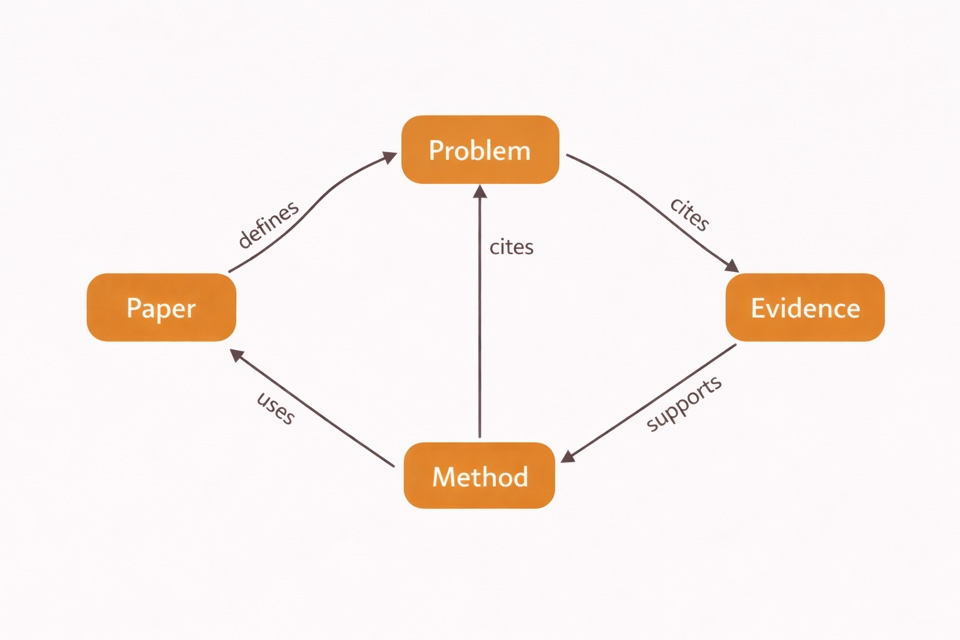
\includegraphics[width=0.82\linewidth, height=0.35\textheight, keepaspectratio]{kg_research.jpg}
	\end{center}

	\note{
Knowledge Graphs offer exactly the structure that RAG lacks --- explicit ontologies, logical relationships, and provenance modeling baked in. Suryawanshi et al. show how this enables cross-document reasoning that vector retrieval simply can't do.

But traditional KGs are high-friction. They require domain experts to curate them manually, they're static snapshots, and they don't evolve as the literature grows. A graph built today is already stale tomorrow.

The gap is automation. We have structure from KGs and we have automation from LLMs --- but they're rarely integrated in a way that lets the graph actually evolve. That integration is exactly what this proposal targets.
	}
\end{frame}

%--- Slide 9: Agentic Systems ---
\begin{frame}
	\frametitle{Agentic Systems}

	\begin{columns}[c]
		\begin{column}{0.63\textwidth}
			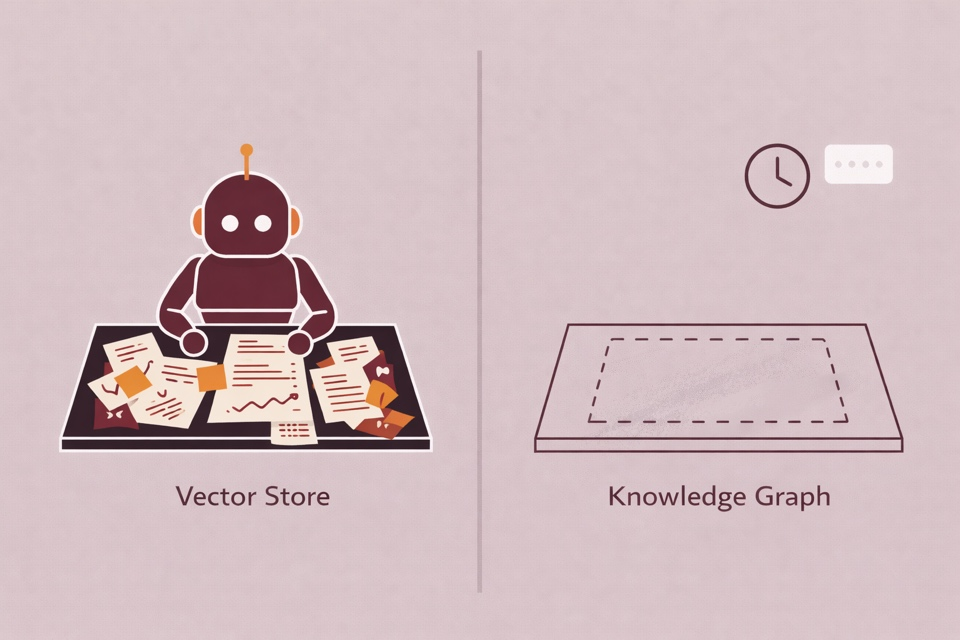
\includegraphics[width=\linewidth]{agentic_amnesia.jpg}
		\end{column}
		\begin{column}{0.34\textwidth}
			\begin{alertblock}{Limitations}
				\begin{itemize}
					\setlength{\itemsep}{4pt}
					\item Ephemeral memory
					\item No structural persistence
					\item Weak auditability
				\end{itemize}
			\end{alertblock}
		\end{column}
	\end{columns}

	\note{
This brings us to Agentic Systems --- projects like Denario and the frameworks Trinkenreich et al. describe. These agents can execute complex, multi-step research tasks. That's genuinely impressive.

But they suffer from amnesia. Memory is bounded by the context window. Once the session ends, the structural state of the research is gone.

There's no persistent substrate anchoring their reasoning over time. Every session starts cold. That's the ceiling we need to break through.
	}
\end{frame}

%--- Slide 10: Empirical Evaluation Standards ---
\begin{frame}
	\frametitle{Empirical Evaluation Standards}

	\begin{columns}[c]
		\begin{column}{0.54\textwidth}
			\begin{itemize}
				\setlength{\itemsep}{6pt}
				\item \textcite{ralph2021empirical}: Empirical Standards for SE
				\item \textcite{baltes2025guidelines}: Guidelines for LLM Studies
			\end{itemize}
			\vspace{0.4em}
			\begin{block}{Observation}
				\small Single-pass or qualitative evaluations dominate.
			\end{block}
			\vspace{0.3em}
			\begin{alertblock}{Need}
				\small Longitudinal evaluation of coherent research state over time.
			\end{alertblock}
		\end{column}
		\begin{column}{0.43\textwidth}
			\centering
			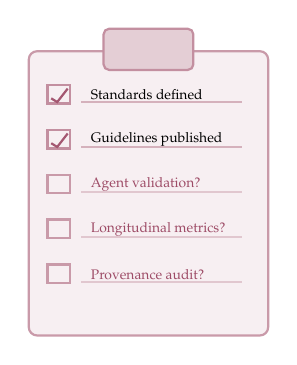
\begin{tikzpicture}[scale=0.95, every node/.style={font=\scriptsize}]
				% Clipboard body
				\draw[rounded corners=3pt, fill=myRed!7, draw=myRed!45, thick] (0,0) rectangle (3.2,3.8);
				% Clip at top
				\draw[fill=myRed!22, draw=myRed!50, thick, rounded corners=2pt] (1.0,3.55) rectangle (2.2,4.1);
				% Row 1: checked
				\draw[draw=myRed!50, thick] (0.25,3.1) rectangle (0.55,3.35);
				\draw[thick, myRed!75] (0.30,3.17) -- (0.38,3.12) -- (0.52,3.30);
				\node[right, font=\tiny] at (0.7,3.22) {Standards defined};
				\draw[myRed!35, thick] (0.7,3.12) -- (2.85,3.12);
				% Row 2: checked
				\draw[draw=myRed!50, thick] (0.25,2.5) rectangle (0.55,2.75);
				\draw[thick, myRed!75] (0.30,2.57) -- (0.38,2.52) -- (0.52,2.70);
				\node[right, font=\tiny] at (0.7,2.62) {Guidelines published};
				\draw[myRed!35, thick] (0.7,2.52) -- (2.85,2.52);
				% Row 3: empty
				\draw[draw=myRed!45, thick] (0.25,1.9) rectangle (0.55,2.15);
				\node[right, font=\tiny, color=myRed!80] at (0.7,2.02) {Agent validation?};
				\draw[myRed!25, thick] (0.7,1.92) -- (2.85,1.92);
				% Row 4: empty
				\draw[draw=myRed!45, thick] (0.25,1.3) rectangle (0.55,1.55);
				\node[right, font=\tiny, color=myRed!80] at (0.7,1.42) {Longitudinal metrics?};
				\draw[myRed!25, thick] (0.7,1.32) -- (2.85,1.32);
				% Row 5: empty
				\draw[draw=myRed!45, thick] (0.25,0.7) rectangle (0.55,0.95);
				\node[right, font=\tiny, color=myRed!80] at (0.7,0.82) {Provenance audit?};
				\draw[myRed!25, thick] (0.7,0.72) -- (2.85,0.72);
			\end{tikzpicture}
		\end{column}
	\end{columns}

	\note{
Finally, how do we evaluate any of this? Ralph et al. and Baltes et al. give us strong standards for SE and LLM experiments --- clear, rigorous, and well-respected in the community.

But current agentic research frequently falls short. Evaluations are single-pass or qualitative. We test a snapshot, not a trajectory.

What's missing is longitudinal evaluation --- frameworks that measure whether an agent is actually maintaining a coherent research state over weeks or months, not just getting the right answer once.
	}
\end{frame}

%---------------------------------------------------------
%	SECTION 3: SYNTHESIS
%---------------------------------------------------------
\section{Synthesis}

%--- Slide 11: Cross-Cutting Gaps ---
\begin{frame}
	\frametitle{Cross-Cutting Gaps in the Literature}

	\begin{columns}[c]
		\begin{column}{0.52\textwidth}
			\centering
			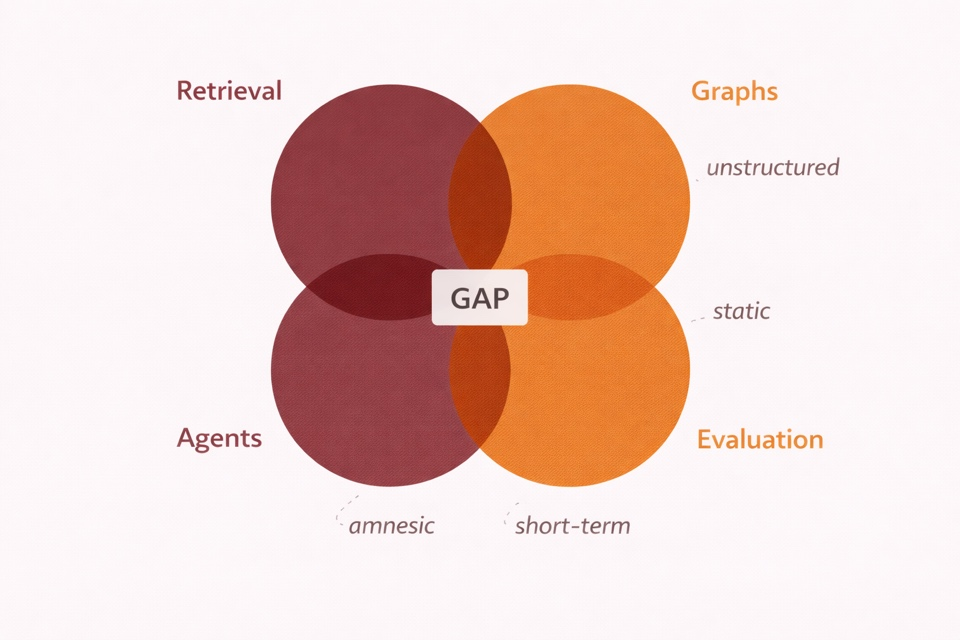
\includegraphics[width=\linewidth, height=0.72\textheight, keepaspectratio]{cross_cutting_gaps.jpg}
		\end{column}
		\begin{column}{0.45\textwidth}
			\begin{itemize}
				\setlength{\itemsep}{8pt}
				\item \textbf{Retrieval} is unstructured
				\item \textbf{Graphs} are static
				\item \textbf{Agents} are amnesic
				\item \textbf{Evaluation} is short-term
			\end{itemize}
			\vspace{0.8em}
			\begin{center}
				\emph{This fragmentation motivates\\new infrastructure.}
			\end{center}
		\end{column}
	\end{columns}

	\note{
Synthesizing across all five domains, the fragmentation is clear.

Retrieval is unstructured. Graphs are static. Agents are amnesic. Evaluation is short-term. Each domain has made real progress in isolation --- but none of them connect.

Retrieval finds content but can't reason over it. Graphs provide structure but require human maintenance. Agents can execute complex tasks but forget everything when the session ends. And our evaluation tools weren't designed for longitudinal, multi-session workflows.

No existing system integrates persistent structured memory with autonomous agency and rigorous provenance. That gap in the center isn't an accident --- it's the core blocker to true AI-assisted research progression.
	}
\end{frame}

%--- Slide 12: Positioning My Work ---
\begin{frame}
	\frametitle{Positioning My Work}

	\begin{block}{Intersection}
		\textbf{Agentic systems} + \textbf{Knowledge graph persistence} + \textbf{Span-level traceability}
	\end{block}

	\vspace{0.4em}
	\begin{columns}[c]
		\begin{column}{0.55\textwidth}
			\textbf{Literature Refined:}
			\begin{itemize}
				\setlength{\itemsep}{5pt}
				\item Stronger empirical evaluation
				\item SE domain scope
				\item Longitudinal validation
			\end{itemize}
		\end{column}
		\begin{column}{0.42\textwidth}
			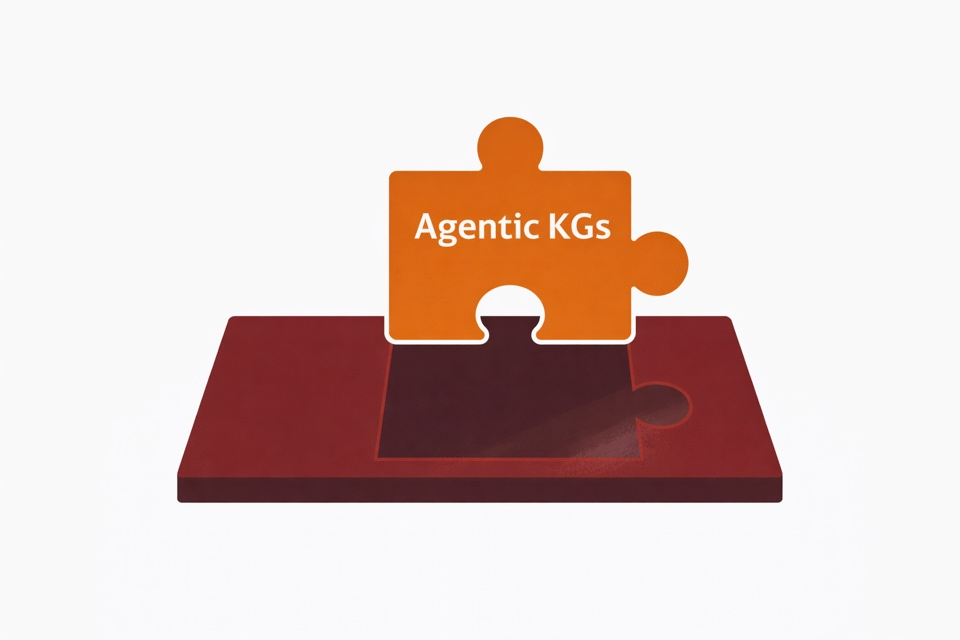
\includegraphics[width=\linewidth, height=0.45\textheight, keepaspectratio]{positioning_my_work.jpg}
		\end{column}
	\end{columns}

	\note{
		My work positions itself directly in the gap we just mapped.

		I'm proposing an architecture at the intersection of three areas: agentic systems, knowledge graph persistence, and span-level traceability. Prior work addresses these in isolation --- RAG scales but lacks structure, knowledge graphs give structure but need manual curation, and agentic systems automate reasoning but suffer from amnesia. My proposal addresses all three simultaneously.

		I also refine the evaluation approach from the literature. Instead of single-pass qualitative assessments, I enforce stronger empirical standards, narrow the scope to software engineering research tasks where the problem is most acute, and introduce explicit longitudinal testing to measure whether the system's knowledge actually persists over time.

		This is not just combining existing tools --- it is defining the infrastructure that makes their combination meaningful, reproducible, and auditable.
	}
\end{frame}

%---------------------------------------------------------
%	SECTION 4: PROPOSAL
%---------------------------------------------------------
\section{Proposal}

%--- Slide 13: Proposed Architecture ---
\begin{frame}
	\frametitle{Proposed Architecture}

	\begin{columns}[c]
		\begin{column}{0.55\textwidth}
			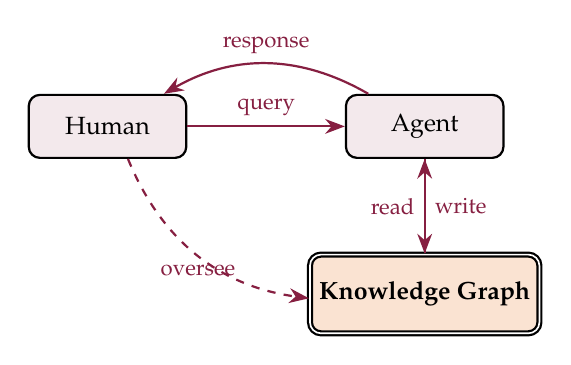
\begin{tikzpicture}[
				node distance=2cm,
				box/.style={draw, rounded corners, fill=myRed!10, minimum width=2cm, minimum height=0.8cm, font=\small, thick},
				kgbox/.style={draw, rounded corners, fill=myOrange!20, minimum width=2.5cm, minimum height=1cm, font=\small\bfseries, thick, double},
				arr/.style={-{Stealth[length=2.5mm]}, thick, myRed}
			]
				\node[box] (human) {Human};
				\node[box, right=of human] (agent) {Agent};
				\node[kgbox, below=1.2cm of agent] (kg) {Knowledge Graph};

				\draw[arr] (human) -- node[above, font=\footnotesize]{query} (agent);
				\draw[arr] (agent) -- node[right, font=\footnotesize]{write} (kg);
				\draw[arr] (kg) -- node[left, font=\footnotesize]{read} (agent);
				\draw[arr, bend right=30] (agent) to node[above, font=\footnotesize]{response} (human);
				\draw[arr, bend right=30, dashed] (human) to node[below, font=\footnotesize]{oversee} (kg);
			\end{tikzpicture}
		\end{column}
		\begin{column}{0.42\textwidth}
			\begin{block}{Persistent Research State Loop}
				\begin{itemize}
					\setlength{\itemsep}{5pt}
					\item Human-in-the-loop oversight
					\item Agent-mediated updates
					\item KG as \textbf{Source of Truth}
				\end{itemize}
			\end{block}
		\end{column}
	\end{columns}

	\note{
		My proposed architecture is a ``Persistent Research State Loop.''

		Instead of a linear chat that disappears after the session, the human and agent collaborate to continuously update a shared, persistent Knowledge Graph.

		The Graph is the source of truth. The agent reads from it to reason about the current state of a research problem, and writes to it to store new conclusions, evidence, and claims. Nothing gets lost between sessions.

		The human stays in the loop --- not just by reading final outputs, but by directly overseeing the state of the graph, correcting errors, and guiding the next query.

		This is the architectural shift: from ephemeral conversation to persistent, structured, auditable research state.
	}
\end{frame}

%--- Slide 13b: Problem Extraction & Ranking ---
\begin{frame}
	\frametitle{Problem Extraction \& Ranking}

	\begin{columns}[c]
		\begin{column}{0.50\textwidth}
			\begin{itemize}
				\setlength{\itemsep}{7pt}
				\item Papers $\to$ problem nodes in KG
				\item Ranked by evidence density \& citation weight
				\item Rank guides agent focus
			\end{itemize}
		\end{column}
		\begin{column}{0.46\textwidth}
			\centering
			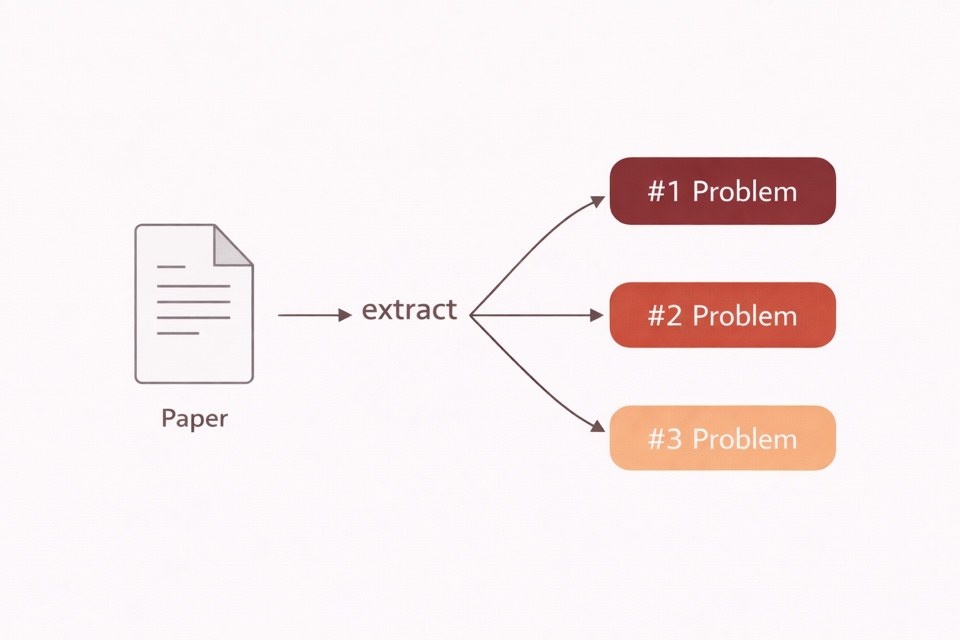
\includegraphics[width=\linewidth, height=0.55\textheight, keepaspectratio]{problem_extraction.jpg}
		\end{column}
	\end{columns}

	\note{
		The agent doesn't just store information --- it actively extracts research problems from ingested documents and represents them as first-class nodes in the Knowledge Graph.

		Those problems are then ranked by how much supporting evidence exists, how frequently they appear across sources, and their citation weight. This ranking is what guides the agent's next action --- what to query, what to write, what to surface to the human.

		It's a lightweight but critical step that turns passive retrieval into directed research progression.
	}
\end{frame}

%--- Slide 14: Core Innovation ---
\begin{frame}
	\frametitle{Core Innovation}

	\begin{center}
		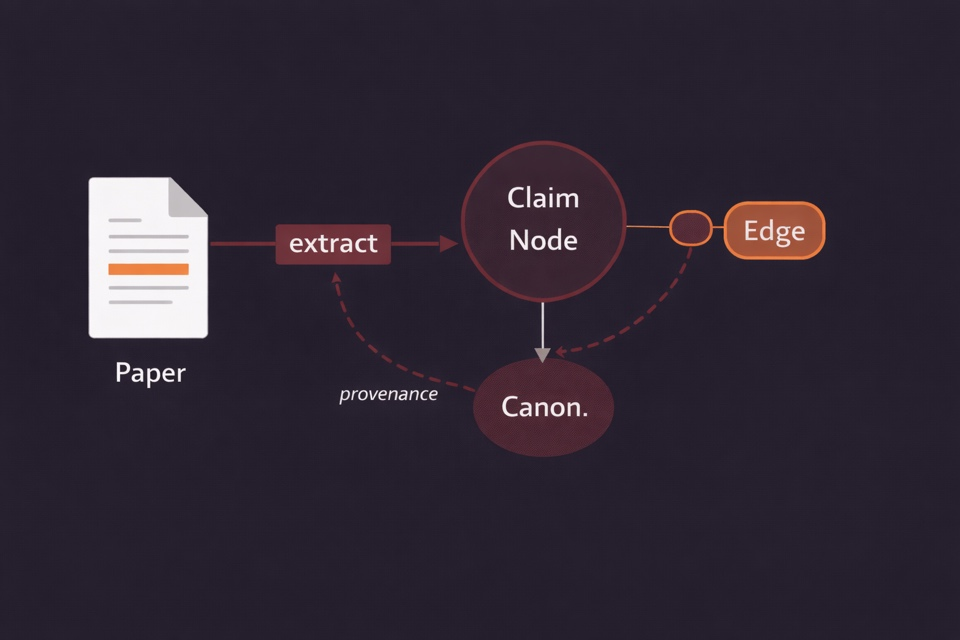
\includegraphics[width=0.80\linewidth, height=0.38\textheight, keepaspectratio]{core_innovation.jpg}
	\end{center}

	\vspace{0.3em}
	\begin{enumerate}
		\setlength{\itemsep}{3pt}
		\item \textbf{Span-level alignment} --- every node traces to a source sentence
		\item \textbf{Canonicalization Agent} --- de-duplicates entities in the graph
		\item \textbf{Versioned provenance chains} --- append-only audit trail
	\end{enumerate}

	\note{
		The core innovation is span-level evidence alignment.

		Standard RAG retrieves vague chunks --- a paragraph, a page, sometimes more. Our architecture links every node and edge in the Knowledge Graph back to the specific sentence or span in the source PDF. You always know exactly where a claim came from.

		We also introduce a Canonicalization Agent whose sole job is to prevent fragmentation --- ensuring we don't end up with five different nodes all representing ``LLM.'' It merges duplicates and keeps the graph clean and queryable.

		Finally, every write to the graph is versioned with a provenance chain --- an append-only log recording the source span, the agent, and the prior graph state. Think of it like a git commit for research knowledge. That's what makes the system reproducible and defensible.
	}
\end{frame}

%---------------------------------------------------------
%	SECTION 5: EVALUATION
%---------------------------------------------------------
\section{Evaluation}

%--- Slide 15: Evaluation Framework ---
\begin{frame}
	\frametitle{Evaluation Framework}

	% Icon bar
	\begin{center}
	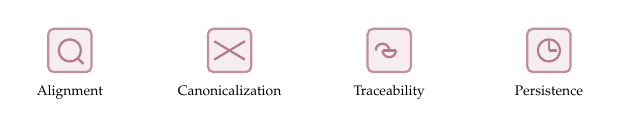
\begin{tikzpicture}[scale=0.78, every node/.style={font=\tiny}, icon/.style={draw, myRed!50, thick, fill=myRed!8, rounded corners=2pt, minimum size=0.55cm}]
		% Magnifier (alignment)
		\node[icon] (i1) at (0,0) {};
		\draw[myRed!60, thick] (0,0) circle (0.18cm);
		\draw[myRed!60, thick] (0.13,-0.13) -- (0.22,-0.22);
		\node[below=0.32cm] at (i1) {Alignment};
		% Merge (canonicalization)
		\node[icon] (i2) at (2.6,0) {};
		\draw[myRed!60, thick] (2.35,0.15) -- (2.6,0) -- (2.85,0.15);
		\draw[myRed!60, thick] (2.35,-0.15) -- (2.6,0);
		\draw[myRed!60, thick] (2.85,-0.15) -- (2.6,0);
		\node[below=0.32cm] at (i2) {Canonicalization};
		% Chain link (traceability)
		\node[icon] (i3) at (5.2,0) {};
		\draw[myRed!60, thick] (4.98,0) arc(180:0:0.11cm);
		\draw[myRed!60, thick] (5.09,0) -- (5.31,0);
		\draw[myRed!60, thick] (5.31,0) arc(0:-180:0.11cm);
		\node[below=0.32cm] at (i3) {Traceability};
		% Clock (persistence)
		\node[icon] (i4) at (7.8,0) {};
		\draw[myRed!60, thick] (7.8,0) circle (0.18cm);
		\draw[myRed!60, thick] (7.8,0) -- (7.8,0.15);
		\draw[myRed!60, thick] (7.8,0) -- (7.93,0);
		\node[below=0.32cm] at (i4) {Persistence};
	\end{tikzpicture}
	\end{center}

	\vspace{0.2em}
	\begin{center}
		\begin{tabular}{@{} l l l @{}}
			\toprule
			\textbf{Claim} & \textbf{Metric} & \textbf{Baseline} \\
			\midrule
			Span-level alignment & Precision / Recall / F1 & Standard RAG \\
			Canonicalization & Cohen's $\kappa$ & Embedding clustering \\
			Traceability & Audit completeness \% & RAG w/ citations \\
			Persistence & Retention accuracy & Chat-only LLM \\
			\bottomrule
		\end{tabular}
	\end{center}

	\vspace{0.1em}
	\begin{block}{Key Question}
		\small Does the system retain knowledge better than a chat-only LLM across multiple sessions?
	\end{block}

	\note{
		To validate the system, I propose a four-claim evaluation matrix.

		For span-level alignment, we measure Precision, Recall, and F1 against human-annotated span labels, with standard RAG as the baseline.

		For canonicalization, we use Cohen's Kappa to measure agreement between the agent's entity merging and expert-labeled canonical clusters.

		For traceability, we audit provenance completeness --- what percentage of graph nodes have unbroken chains back to a source span.

		And the headline metric: persistence. Does the system retain accurate knowledge across multiple sessions, compared to a chat-only LLM that resets each time? That's the claim no prior system has tested longitudinally.

		These four metrics map directly to the four gaps from the literature.
	}
\end{frame}

%--- Slide 16: Experimental Design ---
\begin{frame}
	\frametitle{Experimental Design Overview}

	\begin{columns}[c]
		\begin{column}{0.40\textwidth}
			\begin{itemize}
				\setlength{\itemsep}{8pt}
				\item \textbf{Dataset:} Annotated SE spans
				\item \textbf{Injection:} Synthetic duplicates
				\item \textbf{Audit:} Traceability check
				\item \textbf{Task:} Retention measurement
			\end{itemize}
		\end{column}
		\begin{column}{0.56\textwidth}
			\centering
			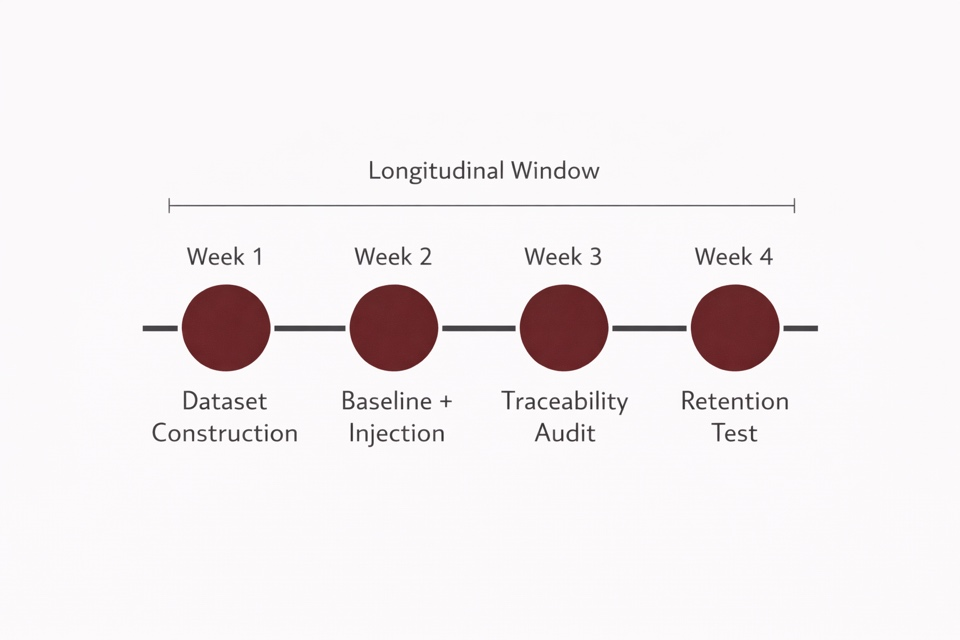
\includegraphics[width=\linewidth, height=0.65\textheight, keepaspectratio]{experimental_design.jpg}
		\end{column}
	\end{columns}

	\note{
		Important context: this evaluation happens \textit{after} the system is built. The qualifier is a research proposal --- this is what we would do to validate the system once implemented.

		The experimental design is a 4-week longitudinal study.

		Week 1: We construct the dataset --- annotated SE papers with human-labeled spans as ground truth.

		Week 2: We run the baseline and inject synthetic duplicates to stress-test the canonicalization agent --- does it correctly merge entities a human would merge?

		Week 3: Human traceability audit --- are provenance chains intact as the graph grows?

		Week 4: The retention test --- we query the system for knowledge ingested in Week 1 and measure whether it retrieves it accurately. This is the longitudinal measurement no prior system has performed.

		Four weeks is the minimum viable window for observing knowledge retention patterns. Ralph et al. and Baltes et al. both flag single-session evaluations as insufficient for systems claiming persistent behavior. The protocol naturally extends to longer periods if needed.

		The full implementation and evaluation sequence is: six months to build a working prototype, followed immediately by this study.
	}
\end{frame}

%---------------------------------------------------------
%	SECTION 6: CONTRIBUTIONS & FUTURE WORK
%---------------------------------------------------------
\section{Contributions}

%--- Slide 17: Contributions ---
\begin{frame}
	\frametitle{Contributions}

	% Three-icon row
	\begin{center}
	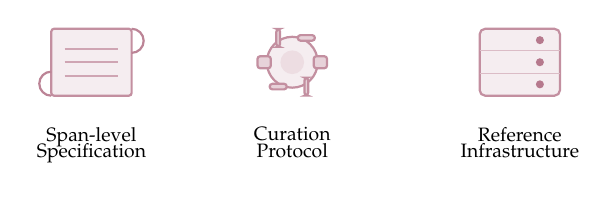
\begin{tikzpicture}[scale=0.85, every node/.style={font=\scriptsize}]
		% Scroll icon (span-level spec)
		\draw[myRed!50, thick, fill=myRed!8, rounded corners=1pt] (0,-0.5) rectangle (1.2,0.5);
		\draw[myRed!40, thick] (0.2,0.2) -- (1.0,0.2);
		\draw[myRed!40, thick] (0.2,0) -- (1.0,0);
		\draw[myRed!40, thick] (0.2,-0.2) -- (1.0,-0.2);
		\draw[myRed!55, thick] (0,-0.5) arc(270:90:0.18);
		\draw[myRed!55, thick] (1.2,0.5) arc(90:-90:0.18);
		\node[below=0.7cm, align=center] at (0.6,0) {Span-level\\[-2pt]Specification};
		% Gear icon (protocol)
		\draw[myRed!50, thick, fill=myRed!8] (3.6,0) circle (0.38cm);
		\draw[myRed!15, thick, fill=myRed!15] (3.6,0) circle (0.16cm);
		\foreach \a in {0,60,120,180,240,300} {
			\draw[myRed!50, thick, fill=myRed!20, rounded corners=1pt]
				({3.6+0.32*cos(\a)-0.09*sin(\a)},{0.32*sin(\a)+0.09*cos(\a)})
				rectangle
				({3.6+0.52*cos(\a)+0.09*sin(\a)},{0.52*sin(\a)-0.09*cos(\a)});
		}
		\node[below=0.7cm, align=center] at (3.6,0) {Curation\\[-2pt]Protocol};
		% Server icon (infrastructure)
		\draw[myRed!50, thick, fill=myRed!8, rounded corners=2pt] (6.4,-0.5) rectangle (7.6,0.5);
		\draw[myRed!30] (6.4,0.17) -- (7.6,0.17);
		\draw[myRed!30] (6.4,-0.17) -- (7.6,-0.17);
		\fill[myRed!60] (7.3, 0.33) circle (0.06cm);
		\fill[myRed!60] (7.3, 0)    circle (0.06cm);
		\fill[myRed!60] (7.3,-0.33) circle (0.06cm);
		\node[below=0.7cm, align=center] at (7.0,0) {Reference\\[-2pt]Infrastructure};
	\end{tikzpicture}
	\end{center}

	\vspace{0.3em}
	\begin{enumerate}
		\setlength{\itemsep}{4pt}
		\item \textbf{Span-level traceability specification} --- foundational vocabulary for the field
		\item \textbf{Agentic Curation Protocol} --- how agents write, update, and validate the KG
		\item \textbf{Reference infrastructure} --- open-source implementation for benchmarking
	\end{enumerate}

	\note{
		The expected contributions are threefold.

		First, a span-level traceability specification --- a precise technical definition of how every claim in the Knowledge Graph links back to its source span. This gives the field the vocabulary it needs to compare systems and measure provenance quality. The working definition of Research State itself is operationalized here: it is the versioned KG of claims, evidence links, and provenance chains.

		Second, an Agentic Curation Protocol --- a concrete specification for how agents should write to, update, and validate a shared knowledge graph. This is the operational layer that makes the architecture reproducible.

		Third, a reference infrastructure implementation --- open-source code and datasets that other researchers can build on, extend, or benchmark against.

		Taken together, these move the field from vague aspiration to concrete, reusable artifacts.
	}
\end{frame}

%--- Slide 18: Near-Term Work ---
\begin{frame}
	\frametitle{Near-Term Work}

	\begin{columns}[c]
		\begin{column}{0.50\textwidth}
			\begin{itemize}
				\setlength{\itemsep}{7pt}
				\item \textit{Months 1--6:} Build system
				\item \textit{Month 6--7:} Evaluation study
				\item \textit{Month 7--8:} Artifact release
				\item \textit{Year 1:} SE deployment
			\end{itemize}
		\end{column}
		\begin{column}{0.46\textwidth}
			\centering
			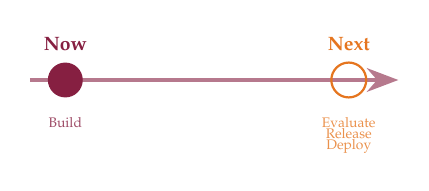
\begin{tikzpicture}[scale=0.9]
				% Road line
				\draw[-{Stealth[length=4mm]}, ultra thick, myRed!60] (0,0) -- (5.2,0);
				% NOW marker
				\fill[myRed] (0.5,0) circle (7pt);
				\node[above=0.25cm, font=\scriptsize\bfseries, myRed] at (0.5,0) {Now};
				\node[below=0.35cm, font=\tiny, align=center, myRed!80] at (0.5,0) {Build};
				% NEXT marker
				\draw[myOrange, thick] (4.5,0) circle (7pt);
				\node[above=0.25cm, font=\scriptsize\bfseries, myOrange] at (4.5,0) {Next};
				\node[below=0.35cm, font=\tiny, align=center, myOrange!80] at (4.5,0) {Evaluate\\[-2pt]Release\\[-2pt]Deploy};
			\end{tikzpicture}
		\end{column}
	\end{columns}

	\note{
		In the near term, my focus is on three sequenced steps.

		Months 1 to 6: build the system --- the KG pipeline, canonicalization agent, and provenance logging layer.

		Month 6 to 7: run the controlled evaluation studies --- the 4-week longitudinal study described on the previous slide.

		Month 7 to 8: release all artifacts openly --- the code, annotated datasets, and evaluation protocol --- so others can reproduce and build on the work.

		Year 1: SE-domain deployment --- a working system applied to real software engineering literature review tasks, validating the proposal in a concrete research context.
	}
\end{frame}

%--- Slide 19: Long-Term Vision ---
\begin{frame}
	\frametitle{Long-Term Vision}

	\begin{columns}[c]
		\begin{column}{0.48\textwidth}
			\begin{itemize}
				\setlength{\itemsep}{6pt}
				\item Cross-domain expansion\newline{\small (Biology, Physics, Climate Science)}
				\item Persistent AI research infrastructure
				\item \textbf{Cross-domain synthesis:} same problem, different fields
			\end{itemize}
		\end{column}
		\begin{column}{0.48\textwidth}
			\centering
			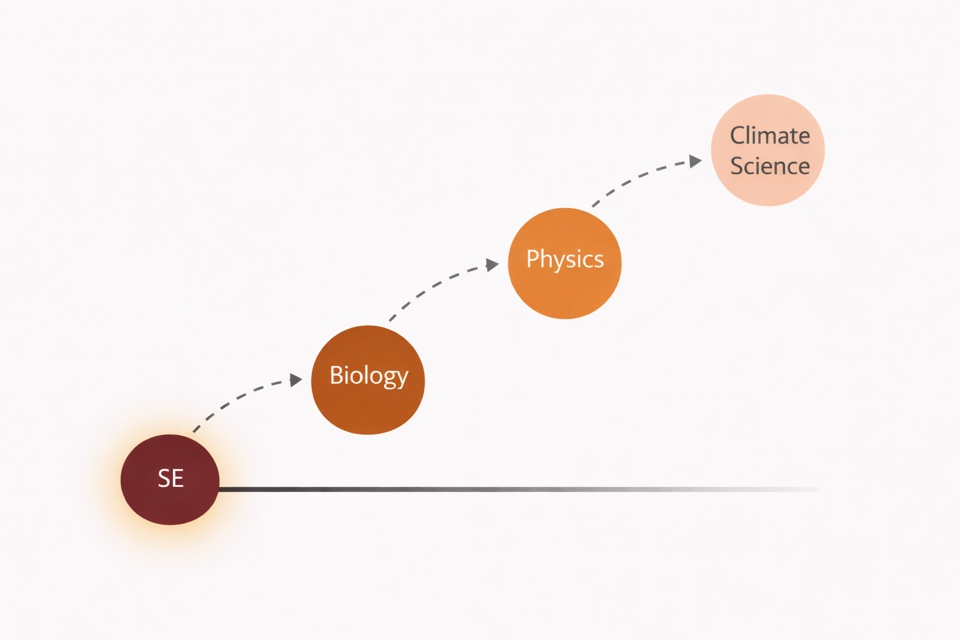
\includegraphics[width=\linewidth, height=0.65\textheight, keepaspectratio]{long_term_vision.jpg}
		\end{column}
	\end{columns}

	\note{
		Long term, this vision extends far beyond Software Engineering.

		Once the architecture is validated in the SE domain, the same infrastructure generalizes to any research discipline that accumulates claims across documents --- Biology tracking experimental hypotheses, Physics linking theoretical claims to simulation evidence, Climate Science connecting model predictions to observational data.

		But the more powerful long-term capability is cross-domain problem synthesis. Once knowledge graphs exist across multiple fields, the system can surface connections that communities would never find on their own. A reproducibility problem in SE may be structurally identical to a chain-of-custody problem in Chemistry, or a simulation provenance problem in Physics --- different vocabulary, different venues, same underlying structure.

		Infrastructure that doesn't just help one field think better, but helps science recognize when it's solving the same problem twice.
	}
\end{frame}

%---------------------------------------------------------
%	SECTION 7: CONCLUSION
%---------------------------------------------------------
\section{Conclusion}

%--- Slide 20: Conclusion ---
\begin{frame}
	\frametitle{Conclusion}

	\begin{columns}[c]
		\begin{column}{0.42\textwidth}
			\begin{itemize}
				\setlength{\itemsep}{6pt}
				\item \textbf{From:} Fragmented, ephemeral chat
				\item \textbf{To:} Persistent, traceable state
				\item \textbf{Goal:} Infrastructure for discovery
			\end{itemize}
			\vspace{0.8em}
			\begin{center}
				\emph{Infrastructure is the missing link\\to autonomous scientific discovery.}
			\end{center}
		\end{column}
		\begin{column}{0.54\textwidth}
			\centering
			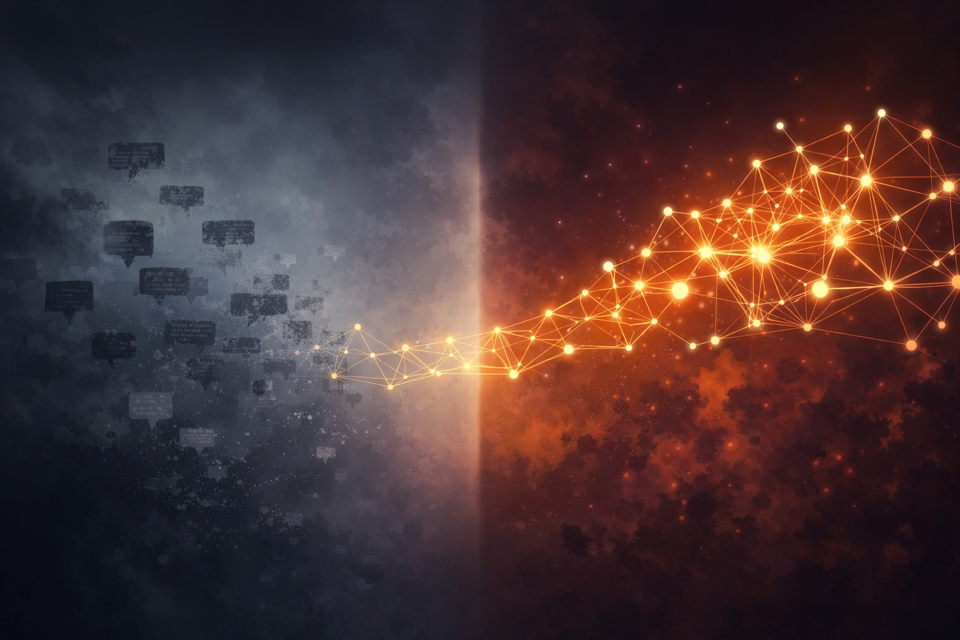
\includegraphics[width=\linewidth, height=0.65\textheight, keepaspectratio]{conclusion_bridge.jpg}
		\end{column}
	\end{columns}

	\note{
		To conclude: we are moving from an era of fragmented, ephemeral chat interactions to an era of persistent, traceable research state --- connected by Agentic Knowledge Graphs as the architectural bridge.

		The core insight from this survey is that the gap in the literature is not a modeling gap. It is an infrastructure gap. Better models will not fix ephemeral memory. Better prompts will not give us span-level provenance. We need architecture that was explicitly designed to persist, trace, and evaluate research state across sessions and across time.

		Infrastructure is the missing link to AI-assisted discovery. That is what this proposal is building.

		Thank you. I am happy to take your questions.
	}
\end{frame}

%---------------------------------------------------------
%	CLOSING SLIDE
%---------------------------------------------------------
\appendix
\setbeamertemplate{headline}{}
\addtobeamertemplate{frametitle}{\vspace*{-\headheight}}{}

\begin{frame}[noframenumbering]
	\begin{center}
		{\LARGE Questions?}

		\vspace{1em}
		{\large Jason Cusati}\\
		\texttt{djjay@vt.edu}
	\end{center}
\end{frame}

%---------------------------------------------------------
%	SEPARATOR
%---------------------------------------------------------
\begin{frame}[noframenumbering, plain]
	\begin{center}
		\vspace{2em}
		{\color{myRed!60}\rule{0.6\textwidth}{0.4pt}}\\[0.8em]
		{\large\color{myRed!80} Backup Slides}\\[0.4em]
		{\color{myRed!60}\rule{0.6\textwidth}{0.4pt}}
	\end{center}
\end{frame}

%---------------------------------------------------------
%	APPENDIX: ANTICIPATED QUESTIONS
%---------------------------------------------------------
% --- Q&A Page 1a: Motivation & Literature (S2, S7, S8) ---
\begin{frame}[noframenumbering]
	\frametitle{Anticipated Questions --- Motivation \& Literature}
	{\small
	\begin{description}[leftmargin=0pt]
		\setlength{\itemsep}{6pt}
		\item[\textbf{Q [S2]: How is Evaluability different from accuracy?}]
			Accuracy measures a single output. Evaluability means the system exposes enough structure to measure \emph{longitudinal} correctness --- whether knowledge degrades, drifts, or accumulates errors across sessions.
		\item[\textbf{Q [S7]: Have you considered hybrid RAG + KG approaches?}]
			Yes --- hybrid systems exist (GraphRAG, etc.) but they use the KG only for retrieval routing, not as an auditable research state. Our contribution is provenance-first: every node is anchored to a source span regardless of retrieval method.
		\item[\textbf{Q [S8]: How does your KG differ from existing domain KGs (Wikidata, biomedical)?}]
			Domain KGs are manually curated, static, and general-purpose. Ours is agent-maintained, append-only versioned, and scoped to the research workflow --- claims link to specific paper spans, not to universal entity definitions.
	\end{description}
	}
\end{frame}

% --- Q&A Page 1b: Literature cont. (S9, S12) ---
\begin{frame}[noframenumbering]
	\frametitle{Anticipated Questions --- Literature (cont.)}
	{\small
	\begin{description}[leftmargin=0pt]
		\setlength{\itemsep}{6pt}
		\item[\textbf{Q [S9]: How does your system avoid the same amnesia you critique?}]
			By externalizing state into the KG. The agent's context window can reset; the graph does not. Every session reads from the graph first, so the agent starts informed, not cold.
		\item[\textbf{Q [S12]: How does this compare to LangChain Memory or MemGPT?}]
			Those frameworks provide session-scoped buffers or rolling summaries --- unstructured, unverifiable, and not provenance-aware. Our KG is structured, auditable, and verifiable against source spans.
	\end{description}
	}
\end{frame}

% --- Q&A Page 2: Architecture & Proposal (S13--S14) ---
\begin{frame}[noframenumbering]
	\frametitle{Anticipated Questions --- Architecture}
	{\small
	\begin{description}[leftmargin=0pt]
		\setlength{\itemsep}{4pt}
		\item[\textbf{Q [S13]: How does human oversight work in practice?}]
			The human reviews the graph state via a query interface --- seeing which claims were added, what spans support them, and flagging incorrect merges. It is not continuous monitoring; it is checkpoint-based review.
		\item[\textbf{Q [S13b]: How do you define a ``research problem'' vs.\ a finding or method?}]
			A problem node captures an open challenge stated or implied in the source. Findings are answers; methods are approaches. The extraction agent uses typed predicates to distinguish them in the ontology.
		\item[\textbf{Q [S14]: How do provenance chains work?}]
			Each KG write records the source span, the agent, and the prior graph state --- like a git commit log. An append-only versioned log; blockchain is a future scaling option.
		\item[\textbf{Q [S14]: Why not just use RAG?}]
			RAG retrieves chunks, not structure. It has no canonical memory, no de-duplication, and no provenance. Our system adds all three.
	\end{description}
	}
\end{frame}

% --- Q&A Page 3a: Evaluation (S15--S16) ---
\begin{frame}[noframenumbering]
	\frametitle{Anticipated Questions --- Evaluation}
	{\small
	\begin{description}[leftmargin=0pt]
		\setlength{\itemsep}{6pt}
		\item[\textbf{Q [S15]: How is your baseline RAG configured --- does it also get citations?}]
			Yes --- the RAG baseline includes citation-level retrieval (RAG w/ citations) so we are comparing against the strongest plausible alternative, not a strawman.
		\item[\textbf{Q [S16]: Why 4 weeks? Why not longer?}]
			Four weeks is the minimum viable window to observe retention patterns; consistent with longitudinal SE field study norms (Ralph, Baltes). The protocol extends naturally to longer periods.
		\item[\textbf{Q [S16]: What's your implementation timeline?}]
			Six months to build a working prototype, followed immediately by the 4-week evaluation study. Artifact release and SE deployment in Year 1.
	\end{description}
	}
\end{frame}

% --- Q&A Page 3b: Contributions (S17--S19) ---
\begin{frame}[noframenumbering]
	\frametitle{Anticipated Questions --- Contributions}
	{\small
	\begin{description}[leftmargin=0pt]
		\setlength{\itemsep}{6pt}
		\item[\textbf{Q [S17]: What does the formal Research State definition look like?}]
			It is operationalized through the architecture: Research State is the versioned KG of claims, evidence links, and provenance chains. Formalizing it as a published specification is Contribution 1.
		\item[\textbf{Q [S18]: What is the biggest technical risk?}]
			Canonicalization quality. If the entity merging agent creates false merges, the graph loses distinguishing structure. The evaluation's Cohen's Kappa check directly stress-tests this.
		\item[\textbf{Q [S19]: How do you handle terminology mismatches across domains?}]
			Cross-domain synthesis is a long-term goal requiring shared ontologies or embedding-based alignment. Near-term, each domain graph uses its own vocabulary; cross-domain linking is deferred to future work.
	\end{description}
	}
\end{frame}

%---------------------------------------------------------
%	SEPARATOR
%---------------------------------------------------------
\begin{frame}[noframenumbering, plain]
	\begin{center}
		\vspace{2em}
		{\color{myRed!60}\rule{0.6\textwidth}{0.4pt}}\\[0.8em]
		{\large\color{myRed!80} References}\\[0.4em]
		{\color{myRed!60}\rule{0.6\textwidth}{0.4pt}}
	\end{center}
\end{frame}

%---------------------------------------------------------
%	REFERENCES
%---------------------------------------------------------
\nocite{trinkenreich2025train}
\nocite{villaescusa2025denario}

\begin{frame}[noframenumbering, allowframebreaks]
	\frametitle{References}
	\printbibliography
\end{frame}

\end{document}
